\documentclass{standalone}
\usepackage{tikz}
\begin{document}
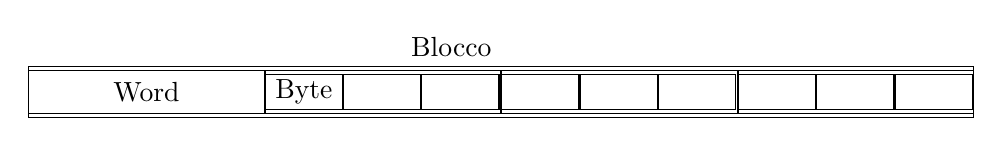
\begin{tikzpicture}
    \draw
    (0,0)node[rectangle, draw, minimum height=0.65cm, minimum width=12cm](b){}
    (b.north)node[above left]{Blocco}
    (b.west)node[rectangle,draw,minimum height=0.55cm, minimum width=2.99cm,anchor=west, inner sep=0](w){Word}
    (w.east)node[rectangle,draw,minimum height=0.55cm, minimum width=2.99cm,anchor=west](w){}
    (w.west)node[rectangle,draw,minimum height=0.45cm, minimum width=0.98cm, anchor=west,inner sep=0](b){Byte}
    (b.east)node[rectangle,draw,minimum height=0.45cm, minimum width=0.98cm, anchor=west,inner sep=0](b){}
    (b.east)node[rectangle,draw,minimum height=0.45cm, minimum width=0.98cm, anchor=west,inner sep=0](b){}
    (w.east)node[rectangle,draw,minimum height=0.55cm, minimum width=2.99cm,anchor=west](w){}
    (w.west)node[rectangle,draw,minimum height=0.45cm, minimum width=0.98cm, anchor=west,inner sep=0](b){}
    (b.east)node[rectangle,draw,minimum height=0.45cm, minimum width=0.98cm, anchor=west,inner sep=0](b){}
    (b.east)node[rectangle,draw,minimum height=0.45cm, minimum width=0.98cm, anchor=west,inner sep=0](b){}
    (w.east)node[rectangle,draw,minimum height=0.55cm, minimum width=2.99cm,anchor=west](w){}
    (w.west)node[rectangle,draw,minimum height=0.45cm, minimum width=0.98cm, anchor=west,inner sep=0](b){}
    (b.east)node[rectangle,draw,minimum height=0.45cm, minimum width=0.98cm, anchor=west,inner sep=0](b){}
    (b.east)node[rectangle,draw,minimum height=0.45cm, minimum width=0.98cm, anchor=west,inner sep=0](b){}
    
    ;
\end{tikzpicture}
\end{document}